
\chapter{Desarrollo del Proyecto}
% [Este capítulo se considera el más importante al elaborar el proyecto de titulación. Se describe el procedimiento seguido para lograr el objetivo planteado. Se explica qué y cómo se hizo, además se debe de convencer de que los métodos o procedimientos usados fueron los más adecuados.

% Deben detallarse los procedimientos, técnicas, métodos, metodologías y demás estrategias metodológicas requeridas para el proyecto.
% ]

En este capítulo se detallará el proceso de diseño e implementación que se realizó para desarrollar el proyecto de monitoreo de estaciones meteorológicas, así como las limitaciones técnicas para el desarrollo de

%! Punto al final de todos los títulos de las imágenes

\section{Producto propuesto}

Se creó un proyecto que permita monitorear el estado de los servicios de las estaciones meteorológicas, así como de la infraestructura en la que dependen, así como ofrecer un control limitado para la solución de problemas de forma remota.


\noindent{El proyecto consiste de tres partes independientes:}

\begin{itemize}
   \item Un módulo para el monitoreo de el \textit{estatus} de las estaciones, que permita el cargar la información de las estaciones de una base de datos, para luego cargar los controladores específicos de cada estación basado en la infrormación existente de las mismas para después guardar el estado en el que se encuentran en una base de datos.

   \item Un API REST que tendrá el objetivo de proveer un acceso sencillo a la información de los sistemas de monitoreo, así como el de proveer una interfaz de control para las estaciones que permita la ejecución remota de comandos preestablecidos, desde cualquier punto con la autorización adecuada que haga una petición a la ruta correspondiente.

   \item Una interfaz gráfica, que permita el acceso a la información correspondiente de los sistemas de monitoreo, así como acceso a los reportes que se generen y permita capturar informes de solución de problemas de las estaciones para su posterior análisis.

\end{itemize}

\section{Metodología de desarrollo}

%? Usar plantilla correcta para el capítulo 3 (Se debe hablar en pasado en capítulo 3)

Para el desarrollo de este programa, se utilizó la estrategia de desarrollo ágil centrada en el usuario. En ella se combina la metodología de desarrollo ágil, la cuál tiene como características principales la entrega continua de resultados y la preferencia de sistemas funcionales sobre documentaciones de código robustas \cite{agile_manifesto}, con el diseño centrado en el usuario, el cuál tiene a los usuarios como objetivo principal para satisfacer las necesidades de requerimientos.

%-? Imagen para ilustrar la metodología de desarrollo ágil
%! Cambiar esta imagen al español
\begin{figure}[!ht]
	\centering
	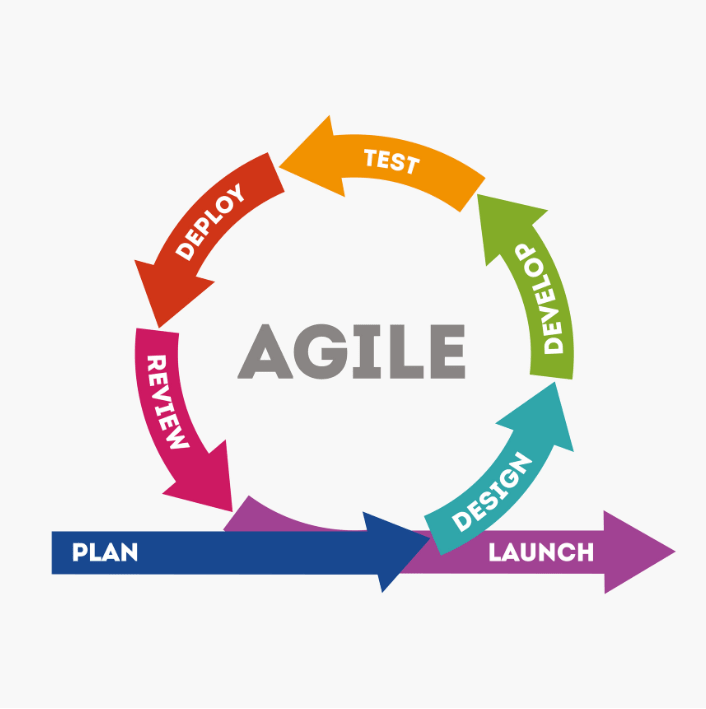
\includegraphics[width=.75\linewidth]{images/agil.png}
	\caption{Diagrama de metodología ágil.}
	\label{fig:agile_methodology}
\end{figure}

Debido a que la experiencia de usuario es uno de los factores que pueden separar al sistema en desarrollo de los sistemas actuales de monitoreo para equipos de cómputo, el esquema de entregas, desarrollo y planeación estarán centrado en el mismo \cite{hussain_agile_usercentered}. El ciclo de entregas será con un sprint de máximo dos semanas, para una revisión de las metas, planeación y objetivos a alto nivel con el usuario y redifinir los requisitos y como sea necesario. La documentación para el usuario final, así como la documentación del API y la información técnica del sistema será un producto que será entregado al finalizar el mismo, apoyándose de la información generada en los sprints.

%? X que se reporta, fue desarrollando utilizando la metodología X y consta de X fase y se realizó X cosa en cada fase. Cada una se explica de forma general.

%? Quitar el siguiente texto, no corresponde a la metodología.

En el respecto del lenguaje de programación, tomando en consideración que la red de monitoreo actual utiliza WeeWX para su integración con estaciones meteorológicas \cite{red_climatologica_uacj}, así como otros componentes del sistema de monitoreo existente, se pretende utilizar Python como lenguaje principal para el desarrollo del núcleo del sistema, sus módulos, y el API de consulta. Para el desarrollo de la interfaz gráfica del sitio web, se elegirá un framework ligero con Javscript. Todo esto se empaquetará en una imagen de Docker para permitir la replicación de la instancia con el mínimo esfuerzo posible.

% \subsection{Programa de Actividades}
%-? Esto está relacionado con la 3.2, debe ser una ssección de la 3.2

%-? Esto es una tabla, no un diagrama. En la tabla X se muestra lo siguiente.
Este proyecto se desarrolló de acuerdo a las actividades que se muestran en la Tabla \ref{Cronograma}.

%! Debido a X y Y, las fases Z se hicieron en X fecha.

{\fontfamily{lmss}\selectfont

%! La tabla no es necesario que vaya en el reporte final

%-? Las tablas deben tener descripción en la parte superior, y debe tener un punto final

\begin{table}[H]
   \centering
   \caption{Actividades a diez meses.}
   \label{Cronograma}
   % \resizebox*{!}{12 cm}{
   \begin{tabular}{|p{8cm}|c|c|c|c|c|c|c|c|c|c|}
      \hline
      ACTIVIDAD&\rotatebox{90}{Febrero 2021}
      &\rotatebox{90}{Marzo}
      &\rotatebox{90}{Abril}
      &\rotatebox{90}{Mayo}
      &\rotatebox{90}{Junio}
      &\rotatebox{90}{Julio}
      &\rotatebox{90}{Agosto}
      &\rotatebox{90}{Septiembre}
      &\rotatebox{90}{Octubre}
      &\rotatebox{90}{Noviembre 2021}\\
      \hline
      Revisión de la Literatura& \checkmark & \checkmark  & \checkmark  &  &  &  &  &  & &  \\
      \hline
      Protocolo&\checkmark &\checkmark  &\checkmark  & \checkmark &  &  &  &  & &  \\
      \hline
      Selección de herramientas & &\checkmark  & \checkmark &  &  &  &  &  & &  \\
      % \hline
      % Documentación de propuesta&  &  & \checkmark & \checkmark &\checkmark  &\checkmark  &\checkmark  &\checkmark  &\checkmark  &\checkmark  \\
      \hline
      Diseño de la interfaz de usuario &  & \checkmark &  &  \checkmark & \checkmark &  &  &  &  &  \\
      \hline
      Documentación de requerimientos &  & \checkmark & \checkmark &  \checkmark & \checkmark &  &  &  &  &  \\
      \hline
      Diseño de la base de datos&  &  &  & \checkmark & \checkmark &  &  &  &  &  \\
      \hline
      Desarrollo del núcleo del sistema&  &  &  &  & \checkmark & \checkmark &  \checkmark &  &  &  \\
      \hline
      Desarrollo de la interfaz de usuario &  &  &  &  &  & \checkmark & \checkmark &  &  &  \\
      \hline
      Desarrollo e implementación del API REST&  &  &  &  &  & \checkmark & \checkmark & \checkmark &  &  \\
      \hline
      Integración con sistema de notificaciones &  &  &  &  &  &  & \checkmark & \checkmark &  &  \\
      \hline
      Compilación y entrega de documentación&  &  &  &  &  &  &  &  & \checkmark & \checkmark \\
      \hline

      Presentación y defensa de trabajo&  &  &  &  &  &  &  &  &  & \checkmark  \\
      \hline
   \end{tabular}
\end{table}
}

\clearpage

\section{Análisis}

Debido a la naturaleza autónoma de las estaciones meteorológicas, y a que el hecho que las mismas se encuentran sometidas a diversos factores que pueden resultar en funcionamiento impredecible, se busca crear un sistema centralizado de recolección de información que tenga gran tolerancia a las diversas condiciones adversas que se enfrentan las estaciones meteorológicas, a la vez que es lo suficientemente confiable para hacer un impacto positivo en la recolección de la información de las mismas.

\subsection{Conexión a estaciones remotas}

%! Si bien puede parecer que el desarrollo de sistemas de monitoreo basados en linux puede tener sus grandes limitaciones. Bash es un lenguaje de programación, y se puede hacer de todo en el.

La conexión a las estaciones remotas se creó como un sistema modular de conexiones. Teniendo el objetivo de la extensibilidad como objetivo prioritario para el sistema de interacción con las interfaces.

Cada sistema de conexión supone sus propios retos, si bien hay diversos métodos de conexión que podrían ser útiles para la conexión a las estaciones meteorológicas, se decidió enfocarse en la conexión vía SSH a las estaciones meteorológicas que poseen una RaspberryPI como \textit{datalogger} y como medio de interfaz que se encuentran conectadas por medio de puerto serial a las mismas. Y de las estaciones meteorológicas Campbell, que poseen diversos protocolos de comunicación pero se decidió por utilizar el protocolo HTTP.

Para la conexión a las estaciones RaspberryPi se considera lo siguiente:

\begin{itemize}
   \item Actualmente cuentan con una VPN configurada para facilitar el acceso a SSH por medio de una dirección IP en el mismo segmento de red que el segmento al que se pretende el servidor final tenga.
   \item Ocasionalmente, las estaciones meteorológicas perderán acceso a la VPN, ya sea por fallas técnicas del servidor, del ISP, pérdidas de energía eléctrica o demás.
   \item Que una estación se encuentre fuera de línea de la VPN temporalmente no implica que esta no pueda operar, o incluso que no pueda contactar al servidor, tal como se observa en la Figura \ref{fig:conexion_redundancia}.
\end{itemize}

\begin{figure}[!ht]
	\centering
	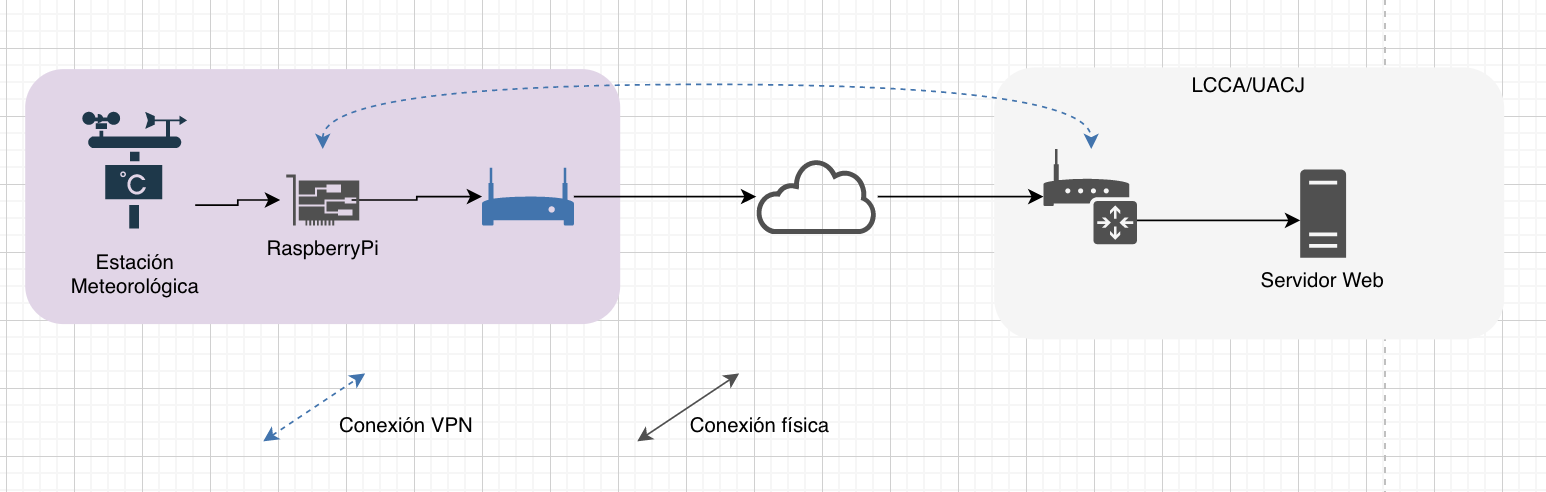
\includegraphics[width=.75\linewidth]{images/diagrams/conexion.png}
	\caption{Diagrama de la redundancia de las conexiones.}
	\label{fig:conexion_redundancia}
\end{figure}

Las estaciones poseen una serie de servicios e información que requiere ser recabada y monitoreada. Si bien, algunas de las estaciones meteorológicas podrían funcionar bajo un plan de datos celulares, los costos actuales de transferencia de datos permiten el no preocuparse tanto por una compresión fuerte de la información transferida.

Los servicios vitales que las estaciones requieren para proporcionar datos de calidad son los siguientes:

\begin{itemize}
   \item El tiempo de la estación.
   \item El servicio de monitoreo climático WeeWX.
   \item Servicios del cliente de VPN para estaciones que así lo requieran.
   \item Servicio de copias de respaldo, como la base de datos (si aplica).
\end{itemize}

% TODO: Cambiar estos a los nuevos servicios monitoreados.

Todos estos procesos y servicios es posible monitorearlos por medio de comandos Bash en la terminal de la estación, por lo tanto, se considera factible monitorearlos de forma adecuada todos para desarrollar este sistema.

\subsubsection{Consideraciones de seguridad}

Debido a que generalmente no se crea una red virtual privada separada para el manejo exclusivo de estaciones meteorológicas (ya que estas suelen instalarse sobre infraestructura existente) es importante tener consideraciones de seguridad respecto a el acceso a las estaciones, debido a que pueden ser un punto de acceso a una, de otra forma, red segura e isolada.

Para realizar la conexión a las estaciones meteorológicas se requiere de acceso a la RaspberryPI que funciona como puente entre ambas. Para realizar cambios, crear un servicio, y establecer la información del sistema con una mínima interacción se requiere de un usuario de alta prioridad a la máquina. En el caso del sistema operativo basado en Linux que utilizan las estaciones, es el usuario con la mayor cantidad de procesos \emph{root}.

Al considerarse comprometido el ambiente de la apliación, se consideraría comprometido el sistema completo. Ya que en este ambiente se encontrarán las contraseñas de acceso a la base de datos y la llave privada que se utiliza para hacer autenticación, si bien existen servicios como AWS-KMS (Key Management Service), el implementar un sistema tan robusto para la administración de secretos sale del alcance de este proyecto.

Por lo tanto, se decidió crear un servicio que tome un usuario y password con acceso \texttt{root} de forma temporal (o al menos uno que tenga permisos de \emph{sudoer}) y utilizarlo para almacenar la llave pública local del servidor para realizar operaciones sin tener un par de usuario y contraseña almacenados en la base de datos que pudiera ser comprometido. De esta forma, se mitiga el impacto de una posible intrusión a la base de datos, y en caso de comprometerse, sólo es es necesario actualizar la llave privada y públicas.

\subsection{Selección de herramientas}

Para el desarrollo de el proyecto, se decidió por realizar la aplicación de servidor con el lenguaje de programación Python. Esto debido a que otros proyectos de los que depende el funcionamiento de los sistemas de el LCCA, tales como el monitoreo climatológico y meteorológico con Weewx, y el proyecto para obtener la información de las estaciones meteorológicas en diferentes estándares \cite{jimenez2019management} fueron realizados con este lenguaje. Además, cuenta con una librería estándar extensa así como una librería de terceras partes madura que permite el desarrollo de forma eficaz utilizando estas librerías existentes, contando con la certeza de que están listas para un proyecto con niveles de producción.

El \textit{ORM} utilizado para el desarrollo de la aplicación, fué \textit{MasoniteORM}, un ORM para Python que tiene como objetivos principales la simpleza y extendibilidad de proyectos. Si bien, \textit{MasoniteORM} es parte de \textit{Masonite}, un framework para el desarrollo de aplicaciones web, este es bastante extenso y complejo, y si bien es fácilmente extensible no es simple para usarse. Por lo tanto, se decidió utilizar el framework de desarrollo de aplicaciones web \textit{FastApi}, creado por Sebastián Ramírez (tiangolo), ya que ofrece una forma fácil de crear un \textit{API} web, el cuál será utilizado posteriormente para el desarrollo de una interfaz fácilmente accesible para los usuarios.

La interfaz gráfica para proveer acceso a la información a los usuarios se decidió hacer en una aplicación web. Esto debido a que las interfaces web ofrecen una amplia y madura plataforma desarrollo que se puede acceder desde diferentes tipos de dispositivos, así como una gran variedad de \textit{frameworks}, metodologías, y paradigmas, lo que ofrece una gran flexibilidad al momento de realizar un desarrollo a la medida. También está el hecho de que debido a la naturaleza del proyecto, un sistema que centraliza toda la información que es accesible por medio de un API, no parecía posible que un proyecto de una aplicación de escritorio o una aplicación web ofreciera una ventaja que no ofreciera la interfaz web.

Para el desarrollo de la interfaz web se optó por el desarrollo con los \textit{frameworks} para desarrollo de aplicaciones web \textit{VueJS} y \textit{TailwindCSS}. Se seleccionó \textit{VueJS} por la cualidad reactiva que posee, la cual permite desarrollar sistemas de monitoreo de información que requieren una constante actualización de los datos sin afectar la experiencia de usuario.

Por el motivo de hacer el proyecto lo más estándar, fácilmente acccesible y mantenible, se decidió realizar la programación y documentación del proyecto en inglés, pero manteniendo las interfaces en las que el usuario interactúa con el mismo en español. Además, se eligió el configurar \textit{pylint} con el estándar \textit{pep8} para el formato automático de el código del proyecto en el estándar. De la misma forma, se configuró \textit{ESLint} en el proyecto de VueJS para el fronted, extendiendo los estándares \textit{vue:essential} y \textit{eslint:recommended}, para realizar el formato automático en los archivos.


\clearpage
\section{Diseño}

Conforme a la metodología de desarrollo centrada en el usuario utilizada en este sistema, se decidió empezar por el desarrollo de un prototipo de alta fidelidad para el diseño del sistema, para posteriormente continuar con el diseño de la infraestructura y los sistemas necesarios para entregar el proyecto, con el objetivo de crear un sistema integral que pudiera satisfacer las necesidades del LCCA al mismo tiempo que cumpliera con los requisitos técnicos necesarios para cumplir los objetivos propuestos.

\subsection{Prototipado de la interfaz gráfica}

Para el desarrollo de un prototipo rápido de la interfaz gráfica, se utilizó el software \textit{Figma}, esto debido a que es un software gratuito, sencillo de utilizar orientado al prototipado de interfaces de alta fidelidad. \textit{Figma} ofrece la capacidad de integrar diferentes \textit{frameworks} de diseño de interfaces, para crear un \textit{design system} (un sistema de diseño) coherente, consistente a través de todo un proyecto. Utilizando este software se decidió utilizar una plantilla de un tablero de control para una plataforma genérica.

Los colores utilizados para el desarrollo de los prototipos, y posteriormente para el desarrollo de la totalidad del proyecto fueron; el color verde \texttt{\#09AB5D} como color principal de la interfaz, debido a su relación con el diseño actual del sitio de consulta de la información de las estaciones meteorológicas, y el color azul \texttt{\#16B2D4} como secundario por su contraste con el color verde y por su actual uso en el sitio existente del LCCA.

Utilizando esta plantilla como base para el lenguaje de diseño de la aplicación, se realizó un prototipado de la interfaz propuesta para evaluar la posible utilidad de la misma, creando un prototipo inicial de alta fidelidad. La primer interfaz en prototiparse fue el tablero de control, después de algunas iteraciones con cambios menores, el prototipo quedó tal como en la Figura \ref{fig:prototype_main_interface}, cabe notar que esta interfaz gráfica tiene elementos en la barra lateral que no corresponden con el proyecto (tal como la sección de chat y otros similares), esto debido a que se dejaron ciertos elementos predefinidos de la plantilla original, para no romper con la estética del diseño.

\begin{figure}[!ht]
	\centering
	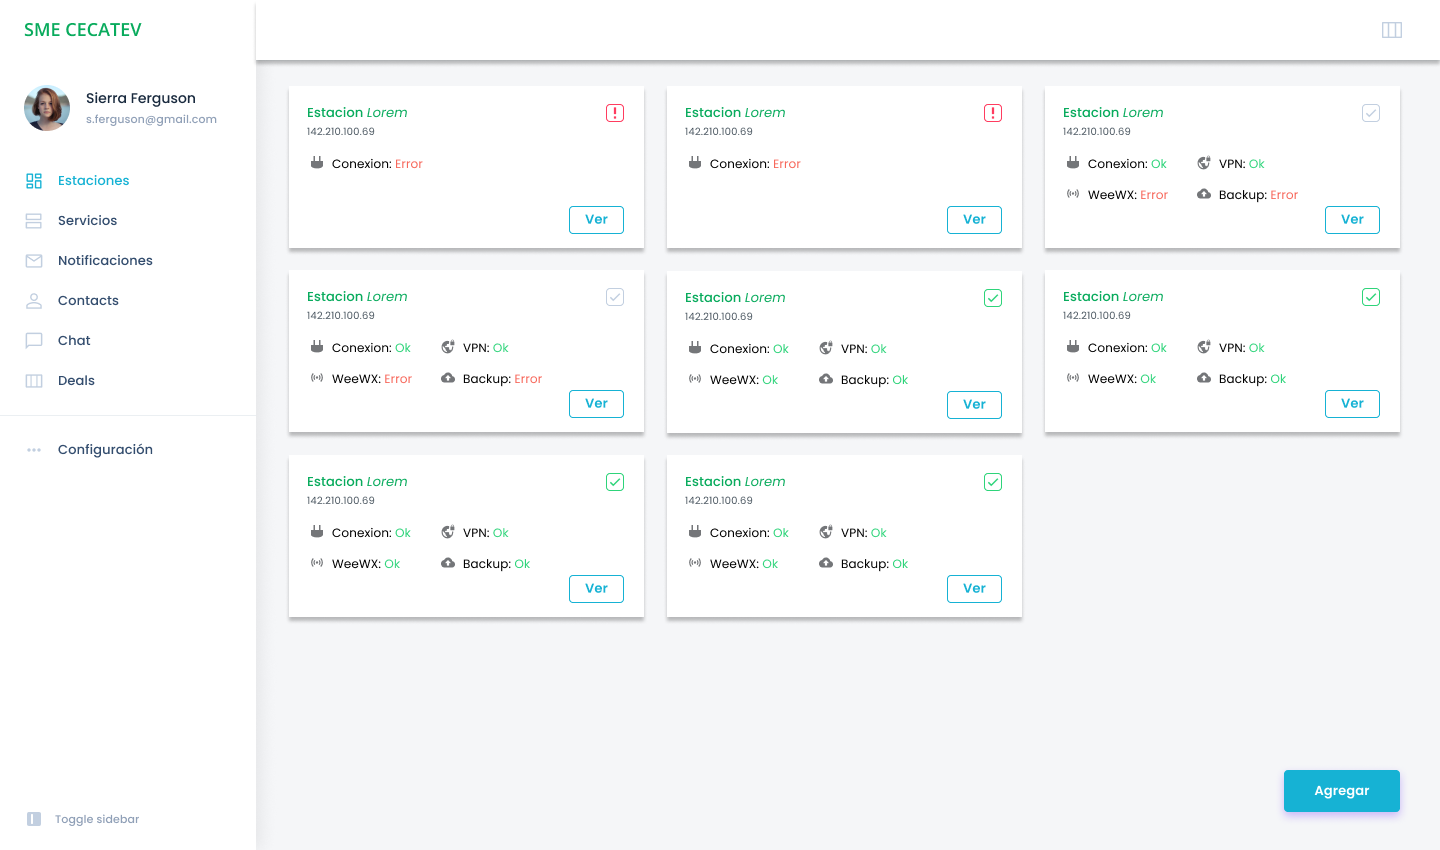
\includegraphics[width=1\linewidth]{images/diagrams/0.0.0_Main_interface.png}
	\caption{Prototipo del tablero de control.}
	\label{fig:prototype_main_interface}
\end{figure}

En este prototipo de interfaz se tomaron en cuenta en varios factores, uno de ellos, es que una estación que es monitoreada puede tener un error de conexión que no permita el acceso a la misma, y que al encontrarse con un error de conexión, no es posible obtener el estado de los servicios. De ser así, la información de estos servicios no se muestra. También se tomó en cuenta el identificar las estaciones por un nombre particular, pero también tener presente la dirección IP de la misma (en caso de poseer una) para volver más sencillo el acceso técnico a la información en caso de ser necesario para un usuario técnico. Además, se hizo la consideración de tener una variedad de diferentes servicios que se podrían monitorear, y que el estado de los servicios y de las estaciones fuera independiente.

\pagebreak

La segunda interfaz que fué elegida para su prototipado, fué la interfaz para agregar una nueva estación meteorológica al sistema. Esta interfaz contiene la información elemental que se requiere para registrar una nueva estación. En este caso, se compone de una dirección IP, un usuario, el método de conexión a la misma, el tipo de estación y el dispositivo por el que se accede a la misma. El prototipo realizado se puede observar en la Figura \ref{fig:prototype_add_station}

\begin{figure}[!ht]
	\centering
	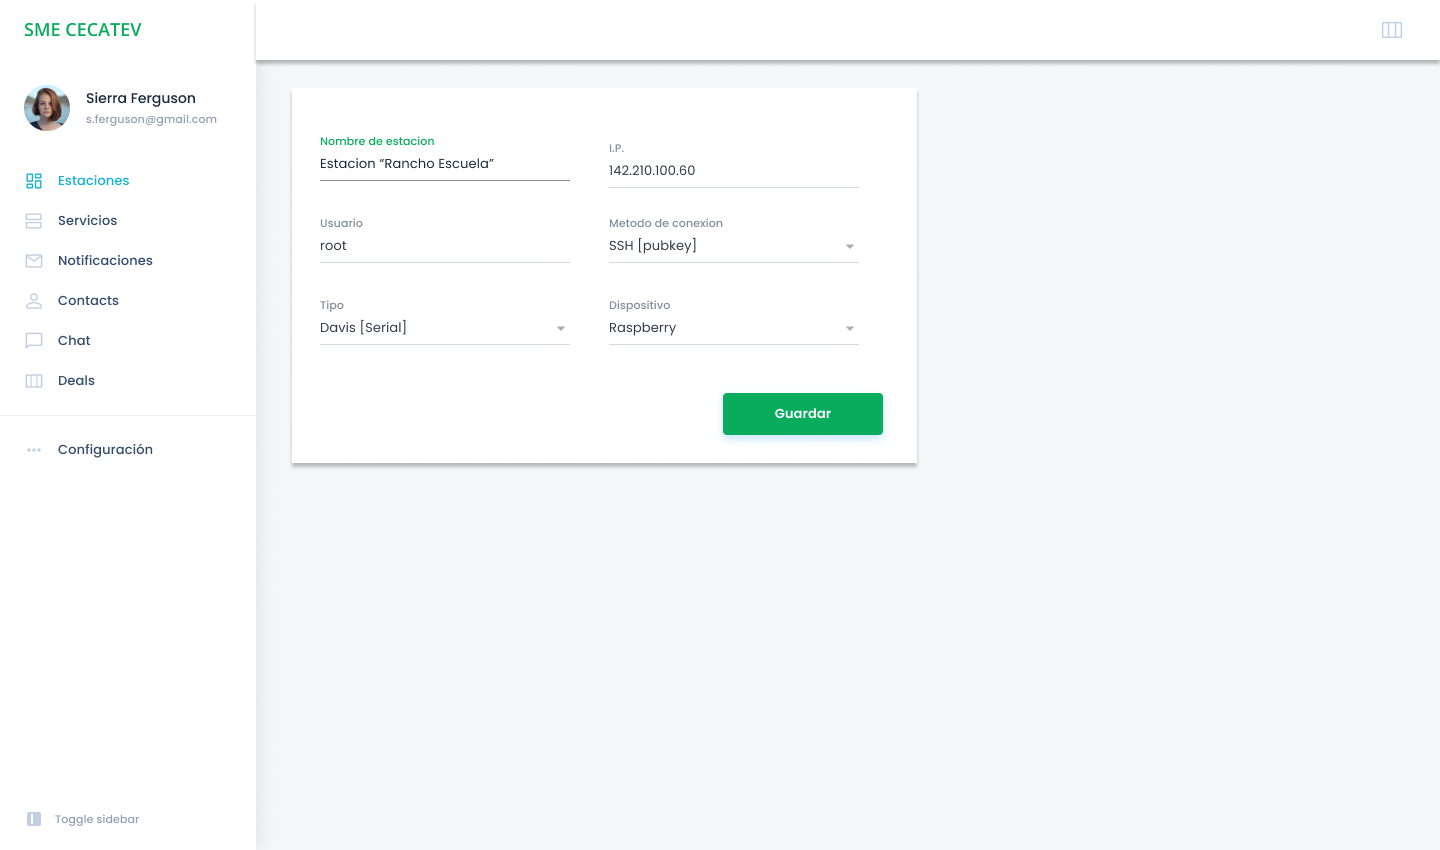
\includegraphics[width=1\linewidth]{images/diagrams/1.0.0_Stations_add.png}
	\caption{Prototipo de la interfaz para agregar una nueva estación.}
	\label{fig:prototype_add_station}
\end{figure}

\pagebreak

Posteriormente se creó el componente de la tercera parte importante del monitoreo de las estaciones meteoreológicas, el prototipo de la interfaz de solución de problemas de las estaciones. Al ser un objetivo secundario importante el poder tener y acceder a la información que las estaciones meteorológicas generan, se considera igualmente importante el poder capturar una razón de la solución de los inconvenientes para futuros análisis. Esta información será capturada con la ayuda de una interfaz como la de la Figura \ref{fig:prototype_solve_error}.

\begin{figure}[!ht]
	\centering
	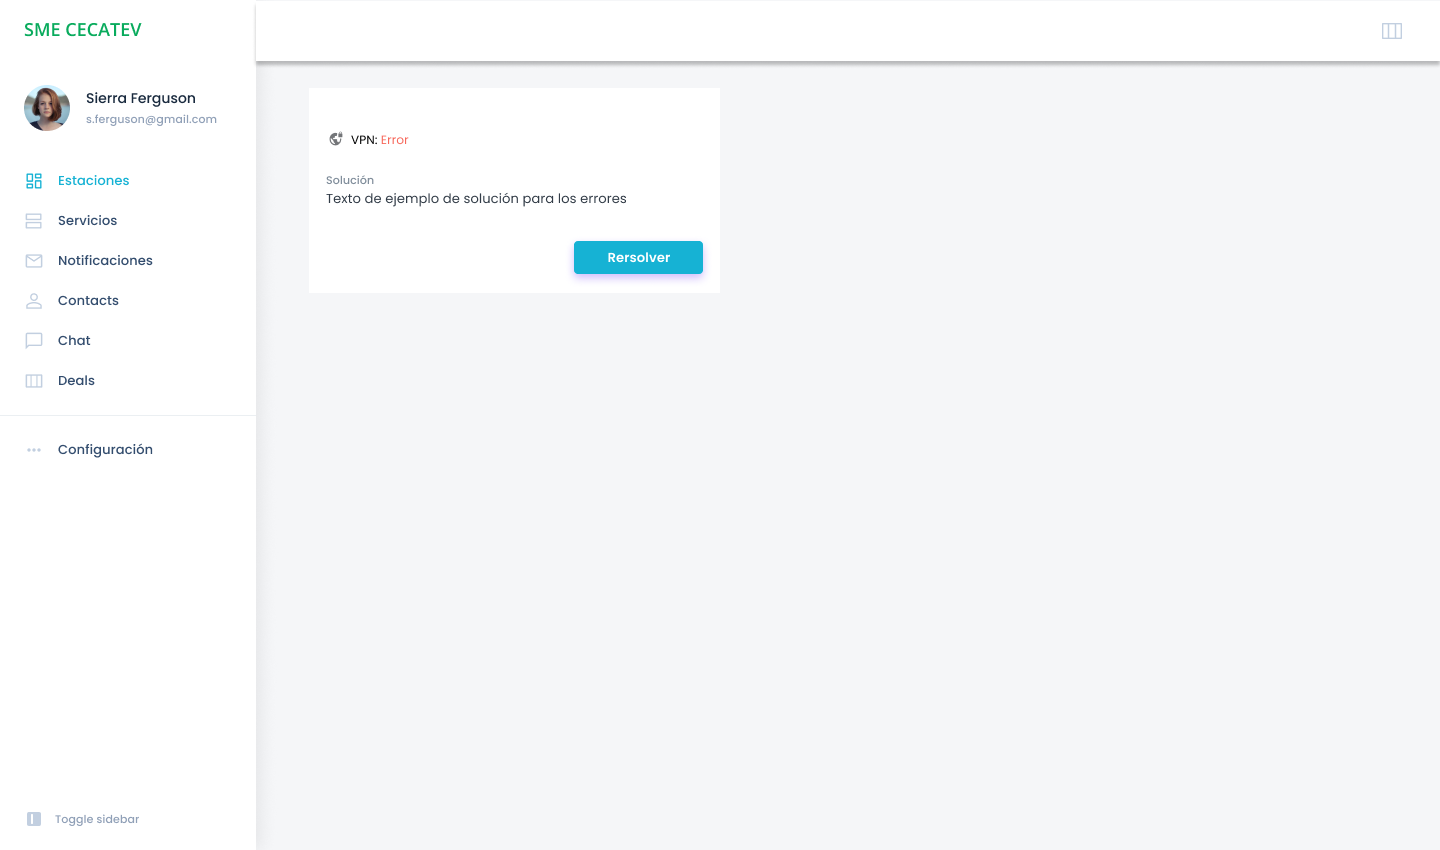
\includegraphics[width=1\linewidth]{images/diagrams/0.1.1_Station_Failing.png}
	\caption{Prototipo de la interfaz de solución de errores.}
	\label{fig:prototype_solve_error}
\end{figure}

\subsection{Diseño de base de datos}

Para el diseño de base de datos del sistema se consideraron dos elementos como relevantes, los datos de las estaciones meteorológicas, que incluyen datos como la conexión a las estaciones y la forma en la que se accederá a ellas, y los eventos que las mismas generen.

Si bien es posible almacenar la información de las estaciones meteorológicas en una \textit{time series database}, en la que la información del estado de cada uno de los servicios y elementos que se monitorean es almacenado sin importar el estado de los mismos, no se considera necesaria la información de los sistemas en su estado funcional, esto debido a que el volumen de datos generado, \textit{O(n*t*s)}, donde \textit{n} es el número de estaciones, \textit{t} la cantidad de veces que la inforamción se consulta por hora y \textit{s} el número de servicios que se consultan, es más grande que la utilidad que se le piensa dar a la información.

La información más relevante que se puede obtener de acuerdo a los objetivos de este proyecto es el estado de las estaciones de monitoreo en caso de falla, así como estimados de la calidad y accesibilidad de los datos que las estaciones recolectan.

Debido a esto, la base de datos se diseñó con el objetivo de almacenar la información en forma de eventos, y tomando en cuenta la utilidad futura de auditoría se decidieron agregar tiempos de creación de eventos y de la solución de los mismos. De la misma forma, el borrado de información no está contemplado en el sistema, para esto se implementó la metodología de borrado de información por medio de \textit{borrados suaves}, los cuales desactivan los registros lógicamente en el sistema sin borrar de forma física los datos de la base de datos.

En cuanto al manejo de la información adicional de las estaciones meteorológicas, es decir, la información de las mismas que no es indispensable para el funcionamiento del sistema pero es necesaria para controles internos, se agregó una tabla de atributos extra. Esta tabla contiene información diversas de las estaciones, y consiste en la forma \textit{llave -> valor} para los campos, esto, para asegurar la mayor flexibilidad posible de los datos y su almacenamiento. Sacrificando velocidades de indexamiento y procesamiento por una mayor libertad para extender y modificar el sistema.

Con todas estas consideraciones en mente, se creó una base de datos que corresponde con los contenidos que se muestran en el modelo entidad-relación que se puede obeservar en la Figura \ref{fig:diagrama_base_de_datos}.

\begin{figure}[!ht]
	\centering
	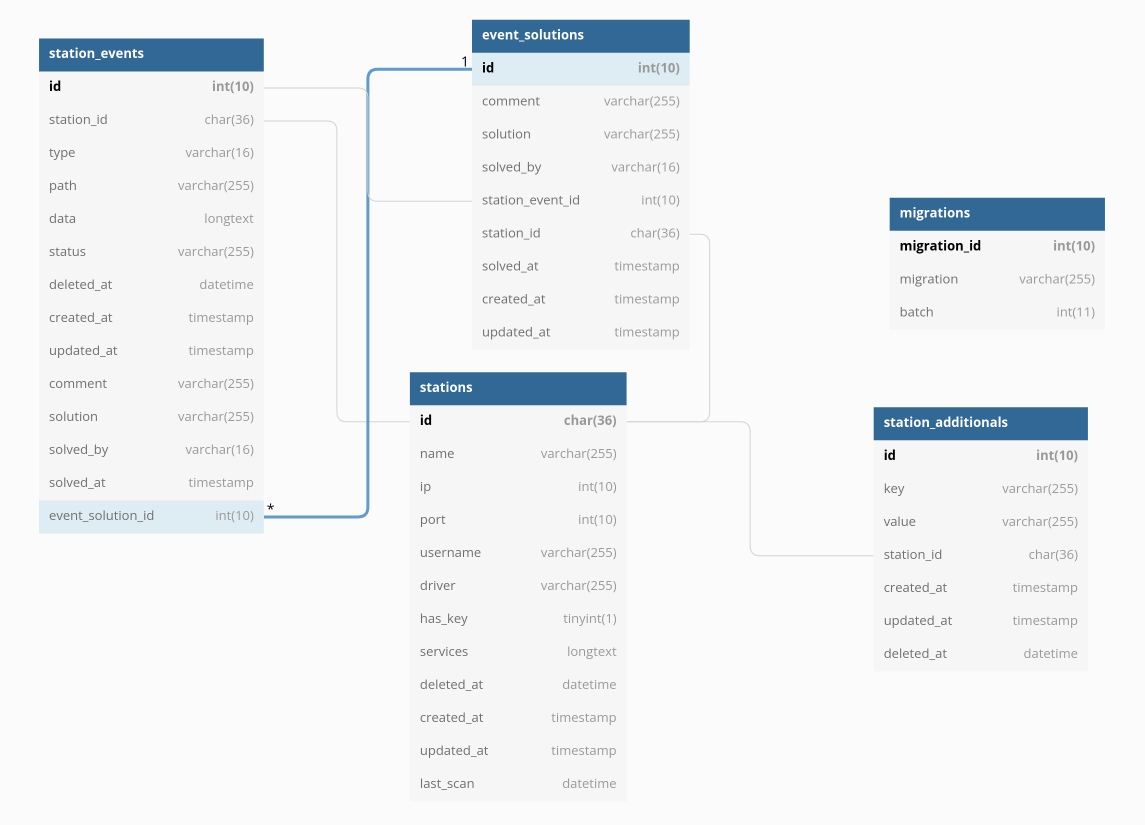
\includegraphics[width=0.86\linewidth]{images/diagrams/database_diagram.png}
	\caption{Modelo entidad-relación del proyecto meteoreo}
	\label{fig:diagrama_base_de_datos}
\end{figure}

\subsection{Arquitectura del sistema}

Para realizar la conexión a las estaciones meteorológicas, se decidió dividir el proyecto en dos componentes principales, un módulo de generación de reportes y un sistema de controladores que contuvieran el código de conexión y restauración de reportes de las estaciones.

Los drivers se desarrollaron con el objetivo de tener una plataforma estándar para la consulta de los datos de las estaciones.

Tomando como referencia el proyecto de \textit{Monitoring Plugins} \cite{monitoring_plugins}, el cual es compatible con diversos proyectos especializados en monitoreo de sistemas de alta resilencia, tales como \textit{Nagios} y \textit{Icinga}, se decidió crear un proyecto basado en drivers fácilmente extendibles.

%! TODO: Todo el desarrollo de la arquitectura del sistema

\subsection{Selección del motor de base de datos}

Para el caso de uso del centro de monitoreo de estaciones meteorológicas de la UACJ, en el que la red actual cuenta con 13 estaciones, no es necesario considerar como cuello de botella el motor de base de datos que se utilizará para el sistema. Esto debido a que, con un tiempo mínimo para la consulta del estado de las estaciones de hasta 5 minutos entre consultas, el sistema podría funcionar incluso con un tiempo promedio de 23 segundos desde la consulta hasta el almacenamiento de la información. Esto, sin tomar en cuenta que es posible paralelizar el proceso de consulta y generación de eventos de las estaciones meteorológicas, por lo que no se considera como algo relevante la selección de un motor de base de datos que cuente con alto rendimiento de lectura y/o escritura de la información.

Debido a que la infraestructura del sistema de las estaciones meteorológicas ya utiliza un motor relacional de base de datos adecuado para el proyecto, MySQL, se pretende utilizarlo para este proyecto, reduciendo la carga de mantenimiento para el equipo de la universidad, además de un sistema familiar que permitirá a los involucrados realizar consultas a la información sin necesidad de aprender nuevas tecnologías.

Para esto, se utilizó la flexibilidad que ofrecen los sistemas modelado de objetos y roles (ORM, por sus siglas en inglés) \cite{Halpin2006}, en la que se permite el crear sistemas agnósticos de un motor de base de datos en específico, y la creación de modelos, esquemas y relaciones de base de datos se dejan al \textit{framework} de modelado de datos. Esto además ofrece soporte para migraciones para realizar actualizaciones de base de datos controladas en caso de requerir extender un sistema existente.

El motor de base de datos seleccionado para el desarrollo local del proyecto fué el conocido como \textit{SQLite}, debido a la flexibilidad que ofrece al ser una base de datos que sólo depende de un archivo para funcionar y que no requiere de instalar paquetes de software extra en la estación que se utiliza para desarrollar y probar el proyecto.

\subsection{Configuración de ambiente de
desarrollo}\label{configuraciuxf3n-de-ambiente-de-desarrollo}

El ambiente de desarrollo que se seleccionó para la sección de python del proyecto fué seleccionado con el objetivo de proveer la mayor flexibilidad y portabilidad a corto y largo plazo, haciendo fácil la modificación posterior del proyecto por los que no estuvieron involucrados inicialmente, y sencillo de replicar para futuras investigaciones. Para lograr estos objetivos, se optó por realizar el proyecto con ayuda de las tecnologías de \textit{Docker}, debido a que permite realizar imágenes de proyectos de forma sencilla, y permite hacer contenedores multiplataforma que con una mínima configuración se vuelven útiles para el desarrollo.

% Con la finalidad de tener un contenedor de desarrollo que pueda ser replicado con la mínima configuración se eligió la plataforma docker, por su amplia adopción y por las facilidades que ofrece para crear sistemas complejos que dependen de varios servicios sin tener que realizar configuraciones en el sistema que puedan ser perdidas al momento de cambiar a otro.

Debido a la sencillez que el sistema de cnfiguración de contenedores \emph{docker compose} ofrece, se eligió para almacenar los parámetros de configuración de los contenedores en vez de crear comandos compatibles con docker para ello. Esto permite una fácil edición de los servicios y la aplicación de los mismos de una forma estandarizada que permite una comprensión más eficaz de los parámetros y de las dependencias.

El archivo de configuración fué almacenado en la raíz del proyecto, con el nombre de \texttt{docker-compose.yml}  tal como el estándar de la utilería \texttt{docker-compose} sugiere, y este archivo tiene el contenido siguiente que se muestra en el listado \ref{lst:docker-compose}. En este archivo, se especifica que se requiere de un servicio de \textit{MySQL}, el cuál fué utilizado para corroborar que el desarrollo era de utilidad con el motor seleccionado para producción, así como una referencia al archivo \textit{Docker} en el que se tiene el contenedor que se utilizará para el desarrollo. Además, se hace referencia a algunas variables, como \texttt{MYSQL\_DATABASE}, que son obtenidas de un archivo \texttt{\.env} estandarizado en la raíz del proyecto.

%! TODO: INSERTAR Referencia de archivo docker-compose en el anterior parrafito
% \begin{listing}
\begin{minted}{yaml}
version: '3.3'
services:
  api:
    container_name: meteoreo-api
    build:
      context: ./
      dockerfile: Dockerfile
    volumes:
      - './:/app:delegated'
    depends_on:
      - mysql
    environment:
      - WEB_CONCURRENCY=2
      - PORT=80
      - PRE_START_PATH=/app/app/prestart.sh
      - GUNICORN_CMD_ARGS="--reload"
    ports:
      - '81:80'
    networks:
      - meteoreo-backend

  mysql:
    image: mysql
    container_name: meteoreo-mysql
    environment:
      MYSQL_DATABASE: '${MYSQL_DATABASE}'
      MYSQL_ROOT_PASSWORD: '${MYSQL_ROOT_PASSWORD}'
      MYSQL_PASSWORD: '${MYSQL_PASSWORD}'
      MYSQL_USER: '${MYSQL_USER}'
      SERVICE_TAGS: dev
      SERVICE_NAME: mysql
    ports:
      - '3306:3306'
    networks:
      - meteoreo-backend

networks:
  meteoreo-backend:
    driver: bridge
\end{minted}
% \caption{Archivo docker-compose}
% \label{lst:docker-compose}
% \end{listing}

El archivo de \textit{docker-compose} tiene una dependencia con un archivo de Docker, que se pretende que facilite la adición de librerías adicionales al proyecto en la posteridad. Actualmente, extiende la imagen existente de \textit{tiangolo}, el proyecto \textit{Uvicorn-Gunicorn-Fastapi}. Esta imagen fue utilizada como base debido a su increíble flexibilidad para el desarrollo de proyectos en FastApi, sus optimizaciones automáticas para el balanceo de cargas entre diversos procesos creados automáticamente (ya que python es monoproceso) y además, por ser una imagen altamente mantenida por la comunidad, debido a su popularidad. En este archivo también se especifíca el instalar la librería \texttt{inteutils-ping} debido a que el proyecto dependerá de realizar pruebas por \texttt{ping} para revisar la conectividad con las estaciones antes de intentar realizar una conexión y la imagen base no tenía esta librería. \ref{lst:dockerfile}.

%! TODO: Insertar referencia de dockerfile en el anterior parrafito

\begin{listing}[h]
\begin{minted}{dockerfile}
FROM tiangolo/uvicorn-gunicorn-fastapi:python3.7

# Installs lib to do pings from the server
RUN apt-get update && apt-get install -y \
   inetutils-ping \
   && rm -rf /var/lib/apt/lists/*

CMD [ "/start-reload.sh" ]
\end{minted}
\caption[Dockerfile]{Archivo Dockerfile}
\label{lst:dockerfile}
\end{listing}

El editor de código seleccionado para el desarrollo del proyecto es Visual Studio Code, el cual posee una gran extensibilidad y predeterminados sensibles que permiten configurar el ambiente de trabajo de la forma que más sea conveniente para el desarrollo del proyecto, además provee la funcionalidad de \textit{devcontainers}, los cuales son parte de una extensión que permiten el crear ambientes de desarrollo dentro de ambientes virtuales en docker, utilizando las herramientas instaladas en la imagen de docker y que no requieren de configuración adicional por parte del desarrollador para comenzar a trabajar en un proyecto. Al detectar un archivo \texttt{devcontainer.json}, esta extensión automáticamente informa al desarrollador de su existencia y le invita a iniciar su ambiente de desarrollo utilizando los parámetros definidos en el arhivo.

En este archivo se especifica un nombre para identificar el ambiente de desarrollo que sea reconocible por el desarrollador, la localización del archivo que describe el contenedor, y una lista de extensiones para el editor de código. Entre las más importantes se encuentra \emph{pylance} que permite  realizar el formato automático de códgo con pep8 y \emph{magicpython} una adición al editor de código que provee un motor de autocompletación para python, las demás siendo preferencias personales útiles para agilizar el desarrollo del proyecto.

%! TODO: Insertar referencia del archivo devcontainer en el parrafito anterior

\begin{minted}{json}
{
  "name": "Meteoreo API",
  "service": "api",
  "remoteUser": "root",
  "shutdownAction": "stopCompose",
  "workspaceFolder": "/app",
  "dockerComposeFile": "../docker-compose.yml",
  "extensions": [
    "editorconfig.editorconfig",
    "mikestead.dotenv",
    "njpwerner.autodocstring",
    "aaron-bond.better-comments",
    "mhutchie.git-graph",
    "hookyqr.beautify",
    "magicstack.magicpython",
    "gruntfuggly.todo-tree",
    "ms-python.vscode-pylance",
    "sleistner.vscode-fileutils"
  ]
}
\end{minted}

Para el desarrollo de la sección de la interfaz de web del proyecto, se instaló en la máquina de desarrollo NPM versión 14.8.1, debido a que era la última versión \textit{LTS} (Soporte a largo plazo, por sus siglas en inglés) disponible, y el sistema de manejo de dependencias \textit{yarn} debido a las ventajas que ofrece sobre \textit{npm}, tales como mayor velocidad de instalación de paquetes y caché multiproyecto. No se vió como un elemento necesario el intergrar Docker o algún otro tipo de tecnología de contenedores para el proyecto de frontend, debido a la ubicuidad de las herramientas y la simpleza de instalación y de mantenimiento de las mismas.


\clearpage

\section{Desarrollo}

Después de haber realizado el análisis inicial de el alcance del proyecto y las necesidades de los usuarios, se comenzó con el desarrollo del proyecto. Este desarrollo se hizo en tres partes. Primero, el desarrollo de un módulo de monitoreo de las estaciones meteorológicas por medio de drivers,  después un API como intermediaria entre la información almacenada en la base de datos y una interfaz gráfica para el monitoreo eficaz.

\subsection{De la base de datos}

Debido a que se seleccionó un sistema basado en un ORM para el manejo de la base de datos, esta tiene que modelarse en el sistema en forma de código para ser reconocida, de la misma forma, la creación de la estructura de la base de datos en el motor se hará por medio de migraciones creadas con el sistema de creación de base de datos, para facilitar su mantenimiento e interoperabilidad en diferentes sistemas y facilitar las integraciones con otros sistemas existentes de información.

Los archivos resultantes de estas migraciones fueron tal como se muestran en el Listado \ref{lst:database-migrations-files}, las cuales se pueden encontrar en la ruta \texttt{/app/database/migrations} del proyecto, tal como es especificado en las guías de desarrollo de MasoniteORM.

\begin{listing}
\begin{minted}{bash}
2021_08_03_052340_stations.py
2021_10_14_162126_station_additional.py
2021_11_13_020934_event_solutions.py            2022_04_03_003436_add_timestamps.py
2021_08_16_000028_station_events.py
2021_10_29_035514_stations.py
2022_03_25_013638_normalize_events_comments.py
2022_04_20_222630_events_fix.py
\end{minted}
\caption{Archivos de migración en el proyecto.}
\label{lst:database-migrations-files}
\end{listing}

Si bien los modelos creados para la ejecución de este proyecto siguen los estándares de modelado de base de datos especificados en MasoniteORM, tal que al modelar la base de datos es posible obtener el mismo código que el implementado, una modificación importante al modelado de los datos es el uso de un mutador para traducir las direcciones IP a enteros y viceversa, como se muestra en el Listado \ref{lst:model-station-mutator}. Este mutador es accesado con un nombre alternativo al nombre del campo en el modelo, debido a que por limitaciones del sistema no es posible utilizar mutadores y accesores con el mismo nombre del campo objetivo.

\begin{listing}
\begin{minted}{python}
import ipaddress
[...]
class Station(Model, UUIDPrimaryKeyMixin, SoftDeletesMixin):
[...]
def get_ip_address_attribute(self):
   return str(ipaddress.ip_address(self.ip))

def set_ip_attribute(self, attribute):
   try:
      ip = ipaddress.ip_address(attribute)
   except ValueError:
      raise ValueError("Invalid IP Address %s" % attribute)

   return int(ipaddress.ip_address(attribute))
\end{minted}
\caption{Definición de accesor y mutador para modelo de estaciones}
\label{lst:model-station-mutator}
\end{listing}

\subsection{Del módulo de monitoreo de las estaciones}

Para realizar la conexión a las estaciones meteorológicas, se decidió dividir el proyecto en dos componentes principales, un módulo de generación de reportes y un sistema de controladores que contuvieran el código de conexión y restauración de reportes de las estaciones.

Tomando como referencia el proyecto de \textit{Monitoring Plugins} \cite{monitoring_plugins}, el cual es compatible con diversos proyectos especializados en monitoreo de sistemas de alta resilencia, tales como \textit{Nagios} y \textit{Icinga}, se decidió crear un proyecto basado en drivers que pudieran ser extendibles. Cada uno de estos drivers, puede cargar una cantidad \textit{n} de módulos o servicios, que contienen la información necesaria para obtener el estado de la estación meteorológica y saber si están funcionando de forma correcta o no.

Con el objetivo de crear un sistema que fuera posible integrar en diferentes ambientes y no requiriera de previa instalación de componentes extra en el dispositivo objetivo, se decidió que la información con la que se revisaría el estado de las estaciones es por medio de un comando que se ejecutaría en una estación remota, o de forma local dado el caso, y se comparara la respuesta obtenida con el resultado de la operación. En caso de que la respuesta de esta operación sea diferente a la respuesta esperada, se buscará en un arreglo de casos conocidos, que pueden ser solucionados con la ejecución de un comando.

La estructura del servicio es un objeto con la forma que se puede apreciar en el Listado \ref{lst:service-example}, donde el arreglo de casos conocidos tiene el nombre de \textit{actions}, y es anidable, lo que permite listar una serie de comandos que pueden ayudar a la solución de problemas con una produndidad \textit{n}.

\begin{listing}
\begin{minted}[%
   breaklines
]{python3}
service = {
   "command": "", # Comando a ejecutar
   "stdout": "", # Salida esperada
   "stderr": "", # Error esperado
   "actions": {
      "read_write_enabled": {
         "response_stdout": "", # Si la respuesta del comando previo es esta
         "response_stderr": "", # Si el error del comando previo es este

         "description": "", # Descripción para el usuario del error
         "solution": "", # Solución propuesta, si existe, para el usuario

         "command": "", # Comando a ejecutar
         "stdout": "", # Salida esperada
         "stderr": "", # Error esperado
         "actions": {
            # ...
         }
      }
   }
}
\end{minted}
\caption{Ejemplo de estructura de un servicio}
\label{lst:service-example}
\end{listing}

Para el desarrollo de la estructura del \textit{driver} de monitoreo de las estaciones meteorológicas, se optó por crear un sistema orientado a la extensión de un componente base que fungiera como sistema principal de ejecución, verificación de credenciales y ejecución de comandos en el sistema objetivo. La estructura de los drivers para el acceso a la información quedó tal como es posible observar en la Figura \ref{fig:diagrama_clase_drivers}.

\begin{figure}[!ht]
	\centering
	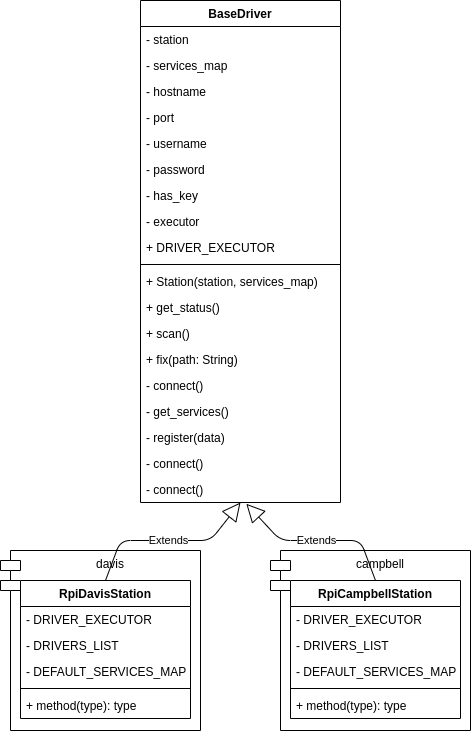
\includegraphics[width=0.2\linewidth]{images/diagrams/classes/drivers.drawio.png}
	\caption{Diagrama de clase de drivers}
	\label{fig:diagrama_clase_drivers}
\end{figure}

Para los ejecutores, tal como se muestra en el diagrama de clases de la Figura \ref*{fig:diagrama_clase_ejecutores}

\begin{figure}[!ht]
	\centering
	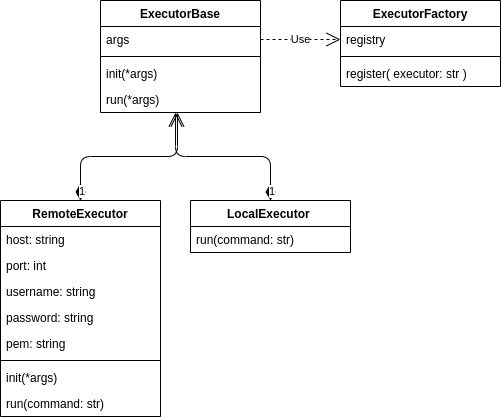
\includegraphics[width=0.6\linewidth]{images/diagrams/classes/executors.drawio.png}
	\caption{Diagrama de clase de ejecutores}
	\label{fig:diagrama_clase_ejecutores}
\end{figure}




\begin{figure}[!ht]
	\centering
	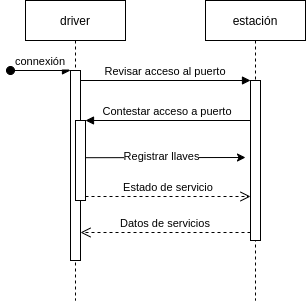
\includegraphics[width=0.5\linewidth]{images/diagrams/classes/registering_execution.drawio.png}
	\caption{Diagrama de clase de drivers}
	\label{fig:diagrama_de_ejecución}
\end{figure}


\subsection{Del módulo de monitoreo de estaciones}

El módulo de monitoreo de estaciones meteorológicas tiene como objetivo el observar la información obtenida por los diversos drivers de conexión a las estaciones meteorológicas y generar reportes conforme sea necesario, la lógica de reporte es tal como se muestra en la figura \ref{fig:logica_de_reporte}.

%! Agregar acciones al diagrama
%! Cambiar por diagrama de secuencia
% Agregar un fin después de generar la alerta
% debe hber un solo inicio y final

\begin{figure}[!ht]
	\centering
	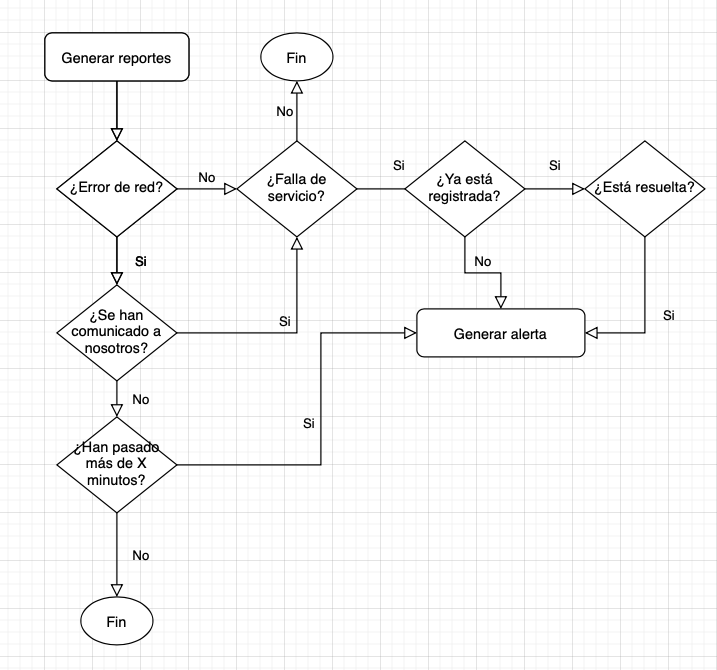
\includegraphics[width=1\linewidth]{images/diagrams/report_logic.png}
	\caption{Lógica de reporte del estado de las estaciones meteorológicas}
	\label{fig:logica_de_reporte}
\end{figure}


\subsection{Del API para el acceso a la información}

\subsection{De la interfaz gráfica del proyecto}

PAra el desarrollo del proyecto, se utilizó tailwind.

\subsection{De la documentación}

Un sistema es tan bueno como su documentación.

\section{Avances}


\section{Módulo de monitoreo}

\subsection*{Requisitos}

\subsection*{Seguridad}

\subsection*{Método de conexion}



\section{Selección de base de datos}

%! Terminar para la próxima

% Casi todas las secciones de desrrollo, van ligadas a una de resultados.

%? Escribir el proceso que realicé. Presentar lo suficiente para darle una idea al lector.

%? Presentar un fragmento de código más relevante. Incluir enlace a repositorio. La funcionalidad se puede expresar en algún tipo de representación gráfica.

%? Evitar párrafos de una sola oración. (Dar MÁS contexto), extranjerismos en itálica.
Con un tiempo de respuesta de $~[N]ms$, el sistema puede soprotar hasta N estaciones concurrentes.

Debido a que la recolección de los datos es por métodología pull y no push, es posible tener las estaciones en una cola que se ejecute hasta por un periodo de 5 minutos (que es un estándar en la recolección de datos de estaciones meteorológicas). Esto implica que la base de datos [X] puede soportar hasta [N x 60 x 5] datos de forma concurrente.

Tomando en cuenta las necesidades actuales del LCCA, y el estimado del tamaño de las redes de alta densidad (que pueden llegar hasta los N nodos como X artículo lo demuestra), no vale la pena el introducir la complejidad extra de un motor de base de datos desconocido y para el que no existen ORM's con soporte completo en el lenguaje de desarrollo. Porque no es un sistema de alta densidad de datos.

Si bien es posible escalar horizontalmente la infraestructura, se busca evitarlo ya que los \textit{diminishing returns} del costo de tener que mantener un sistema de monitoreo no es costeable. Para los casos de sistemas de extremadamente alta densidad, se recomienda el crear varias instancias seccionadas en bases de datos, o escalar la base de con un redis en vez de escalar.

%! Recordar que la información debe ser consultada desde el API, así que no sólo se tienen que tomar en cuenta la cantidad de query's por segundo que se requieren hacer para las inserciones, sino también para la consulta de datos.

%! Si lo que queremos es proveer herramientas para la gestión de calidad de los datos meteorológicos, la información tiene que tener en mente los principios Solidos y transaccionales, al menos en la creación de reportes basados en incidentes.

\subsection{Selección del motor de base de datos}

Para el caso de uso del centro de monitoreo de estaciones meteorológicas de la UACJ, en el que la red actual cuenta con 13 estaciones, no es necesario considerar como cuello de botella el motor de base de datos que se utilizará para el sistema. Esto debido a que, con un tiempo mínimo para la consulta del estado de las estaciones de hasta 5 minutos entre consultas, el sistema podría funcionar incluso con un tiempo promedio de 23 segundos desde la consulta hasta el almacenamiento de la información. Esto, sin tomar en cuenta que es posible paralelizar el proceso de consulta y generación de eventos de las estaciones meteorológicas, por lo que no se considera como algo relevante la selección de un motor de base de datos que cuente con alto rendimiento de lectura y/o escritura de la información.

Debido a que la infraestructura del sistema de las estaciones meteorológicas ya utiliza un motor relacional de base de datos adecuado para el proyecto, MySQL, se pretende utilizarlo para este proyecto, reduciendo la carga de mantenimiento para el equipo de la universidad, además de un sistema familiar que permitirá a los involucrados realizar consultas a la información sin necesidad de aprender nuevas tecnologías.

Para esto, se utilizó la flexibilidad que ofrecen los sistemas modelado de objetos y roles (ORM, por sus siglas en inglés) \cite{Halpin2006}, en la que se permite el crear sistemas agnósticos de un motor de base de datos en específico, y la creación de modelos, esquemas y relaciones de base de datos se dejan al \textit{framework} de modelado de datos. Esto además ofrece soporte para migraciones para realizar actualizaciones de base de datos controladas en caso de requerir extender un sistema existente.

El motor de base de datos seleccionado para el desarrollo local del proyecto fué el conocido como \textit{SQLite}, debido a la flexibilidad que ofrece al ser una base de datos que sólo depende de un archivo para funcionar y que no requiere de instalar paquetes de software extra en la estación que se utiliza para desarrollar y probar el proyecto.

